% Comentar a integração entre automotiva e eletronica

\section{Automotiva e Eletrônica} % (fold)
\label{sec:automotiva_e_eletr_nica}

No intuito de obter os melhores resultados dos sensores e mantendo a conservação da estrutura da bicicleta, a equipe de eletrônica em consulta com o resto do grupo e em especial com a equipe de automotiva, estudou o posicionamento dos sensores de forma a obter os melhores resultados  possíveis sem a alteração na estrutura.

Uma das medidas discutidas para a captura da direção que o usuário deseja da bicicleta foi o aproveitamento do parafuso centrado do guidão em conjunto com uma segueta para a alteração da posição do potenciômetro. A \autoref{fig:figuras_experimentos_img_20141128_wa0013} apresenta o detalhe do posicionamento da segueta com o parafuso já posicionado.

\begin{figure}[h]
  \centering
	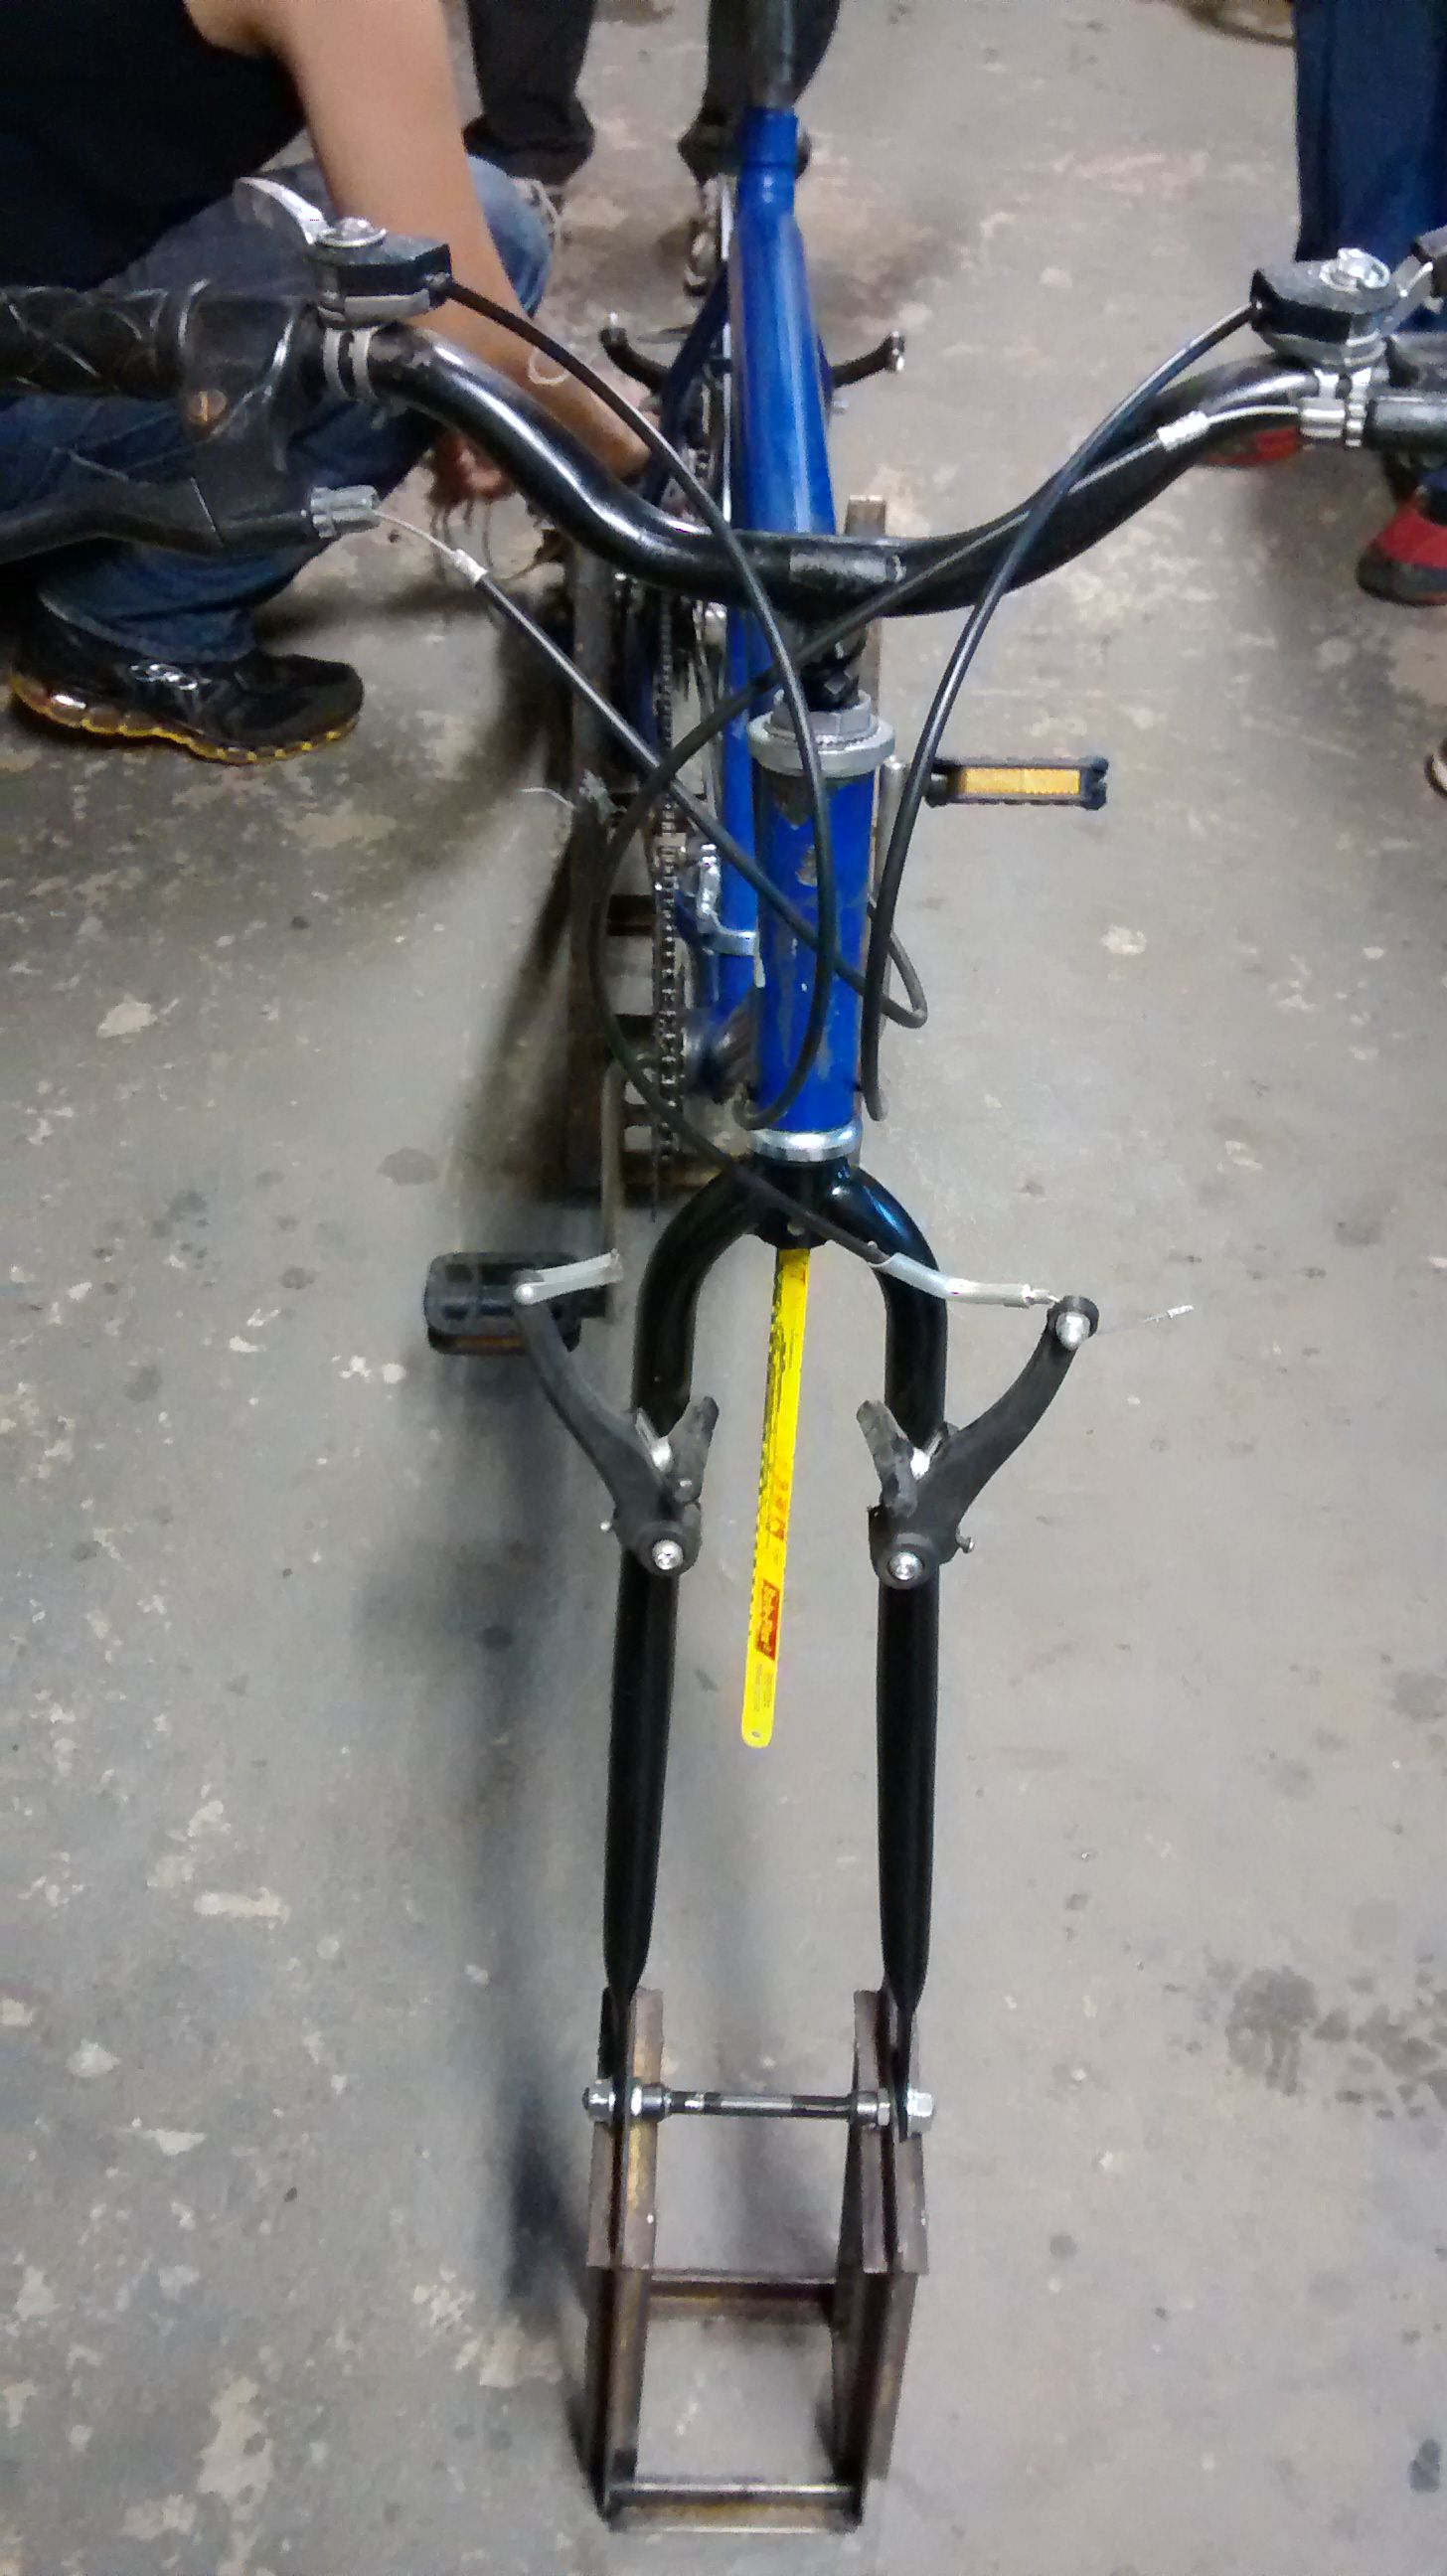
\includegraphics[width=0.3\textwidth]{figuras/experimentos/IMG-20141128-WA0013}
  \caption{Detalhe para a captura da direção da bicicleta}
  \label{fig:figuras_experimentos_img_20141128_wa0013}
\end{figure}

Para o posicionamento do potenciômetro, será fixada uma barra de ferro nos parafusos dos freios dianteiros, como mostra a \autoref{fig:figuras_experimentos_img_20141201_102632506}.


\begin{figure}[h]
  \centering
	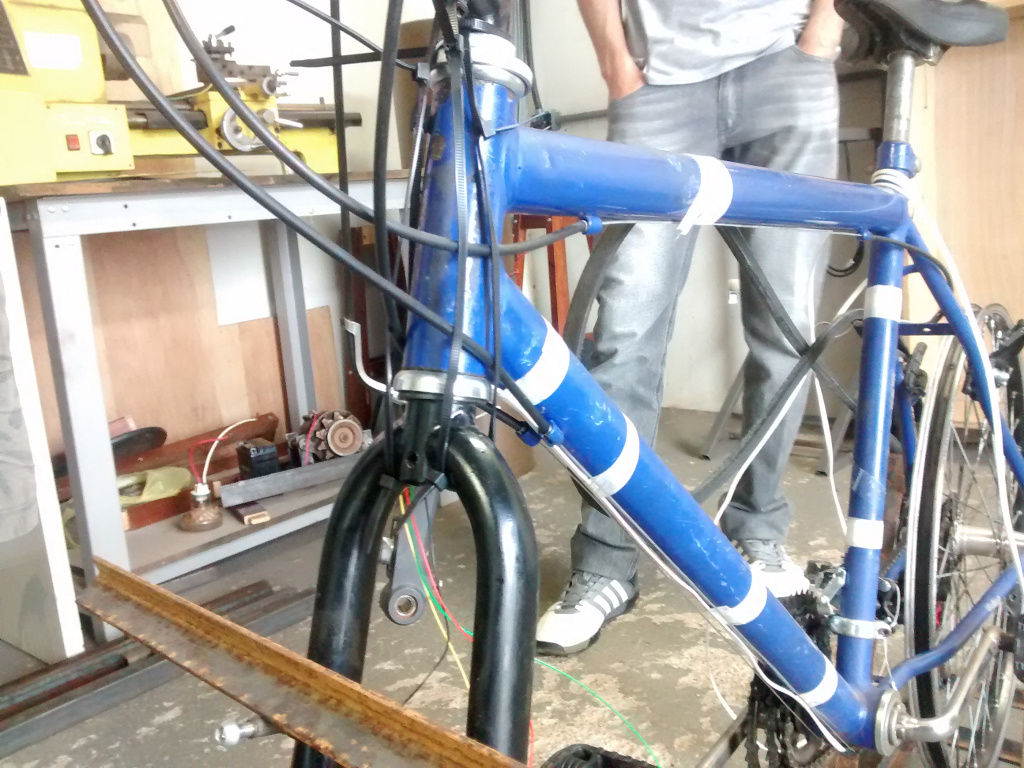
\includegraphics[width=0.8\textwidth]{figuras/experimentos/IMG_20141201_102632506}
  \caption{Detalhe do posicionamento do suporte para o potenciômetro.}
  \label{fig:figuras_experimentos_img_20141201_102632506}
\end{figure}

Para o posicionamento do servo motor, foi projetado um suporte posicionado próximo ao freio traseiro, detalhe na \autoref{fig:figuras_experimentos_10822582_753173958090872_1775024898_n}, de forma a tracionar o cabo de aço quando indicado pelo programa para indicar a sensação de peso ao pedalar a bicicleta.


\begin{figure}[h]
  \centering
	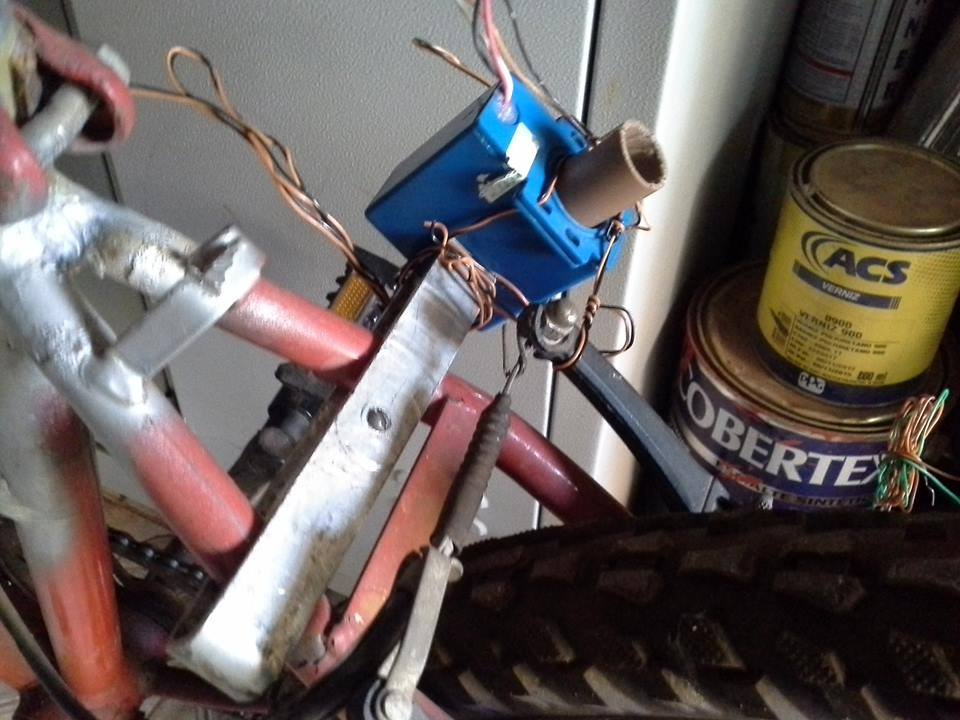
\includegraphics[width=0.8\textwidth]{figuras/experimentos/10822582_753173958090872_1775024898_n}
  \caption{Detalhe para suporte do servo motor}
  \label{fig:figuras_experimentos_10822582_753173958090872_1775024898_n}
\end{figure}



Os circuitos descritos na \autoref{sec:circuito} foram soldados numa placa que pode ser visualizado por meio da \autoref{fig:placa_sensores}. Os pinos foram posicionados de forma ficarem na extremidade direita da placa. Isso proporciona maior facilidade de nas conexões entre a placa do Arduino. Todos os fios com o sinal de saída dos sensores foram unidos com fitas, pois a placa foi alocada junto ao Arduino. 

\begin{figure}[!htb]
        \centering
        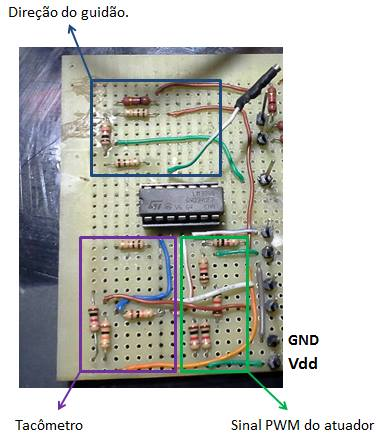
\includegraphics[width=0.7\textwidth]
{figuras/10822194_753168071424794_1809189156_n.jpg}
        \caption{Placa com os circuitos dos sensores.}
        \label{fig:placa_sensores}
\end{figure}

Os sensores do tacômetro foram posicionados no cruzamento entre dois raios da bicicleta, como pode ser observado na \autoref{fig:figuras_experimentos_img_20141201_120657817}. Isso se deve ao fato deste cruzamento apresentar maior área, fazendo com que a interrupção do sensor infravermelho seja mais pronunciante o que proporciona uma leitura mais precisa.


\begin{figure}[!htb]
  \centering
	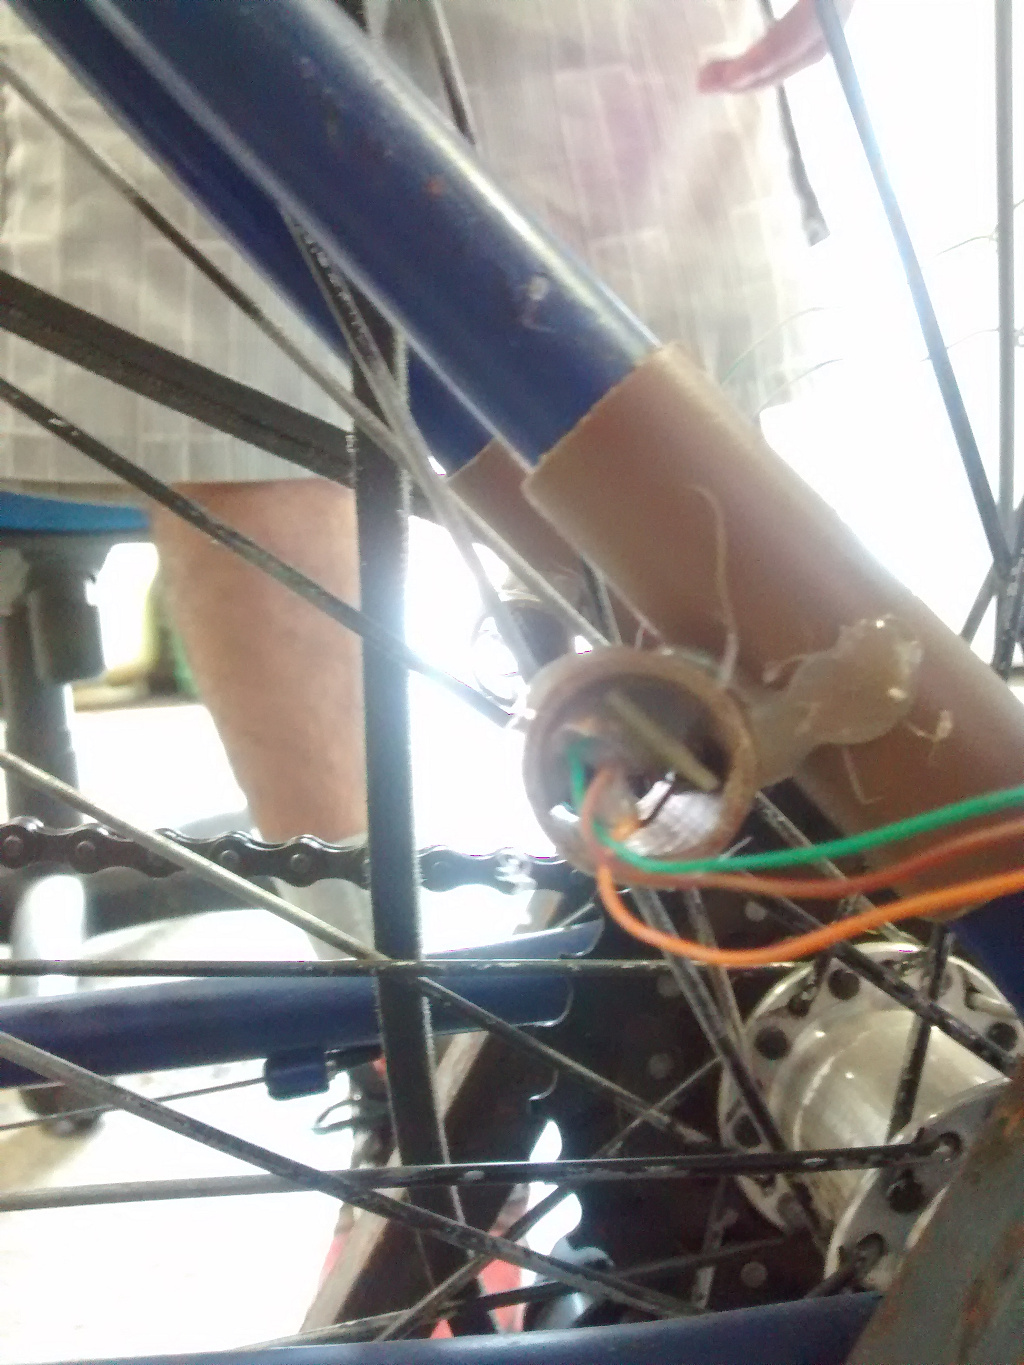
\includegraphics[width=0.5\textwidth]{figuras/experimentos/IMG_20141201_120657817}
  \caption{Detalhe do posicionamento do tacômetro}
  \label{fig:figuras_experimentos_img_20141201_120657817}
\end{figure}